\documentclass[tikz]{standalone}

\usepackage{tikz}
\usetikzlibrary{backgrounds}

\usepackage{amsmath}

\newcommand{\tp}{^T}

\begin{document}

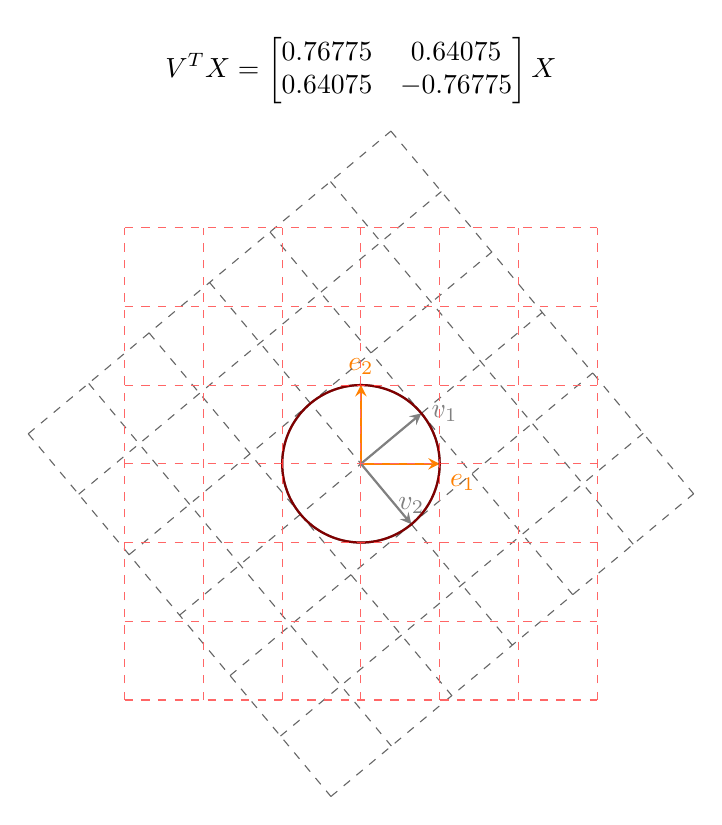
\begin{tikzpicture}% {{{ V^T X
	\node at (0, 5){$V\tp X =\begin{bmatrix}  0.76775 & 0.64075 \\ 0.64075 & -0.76775  \end{bmatrix} X $};
	\pgftransformcm{0.76775}{0.64075}{0.64075}{-0.76775}{\pgfpoint{0}{0}}
	\draw [thin,black!60, dashed] (-3,-3) grid (3,3);
	\draw[thick, ->, >=stealth, gray] (0,0) -- +(1,0) node[right]{$v_1$};
	\draw[thick, ->, >=stealth, gray] (0,0) -- +(0,1) node[above]{$v_2$};
	\draw[thick] (0,0) circle (1);


	\pgftransformcm{0.76775}{0.64075}{0.64075}{-0.76775}{\pgfpoint{0}{0}}
	% \pgftransformcm{0.85065}{0.52573}{-0.52573}{0.85065}{\pgfpoint{0}{0}}
	\draw [red!60, thin, dashed] (-3,-3) grid (3,3);
	\begin{scope}[on background layer]
		\draw[thick, ->, >=stealth, orange] (0,0) -- +(1,0) node[below right]{$e_1$};
		\draw[thick, ->, >=stealth, orange] (0,0) -- +(0,1) node[above]{$e_2$};
	\end{scope}
	\draw[thick, red, opacity=0.5] (0,0) circle (1);
\end{tikzpicture}% }}}

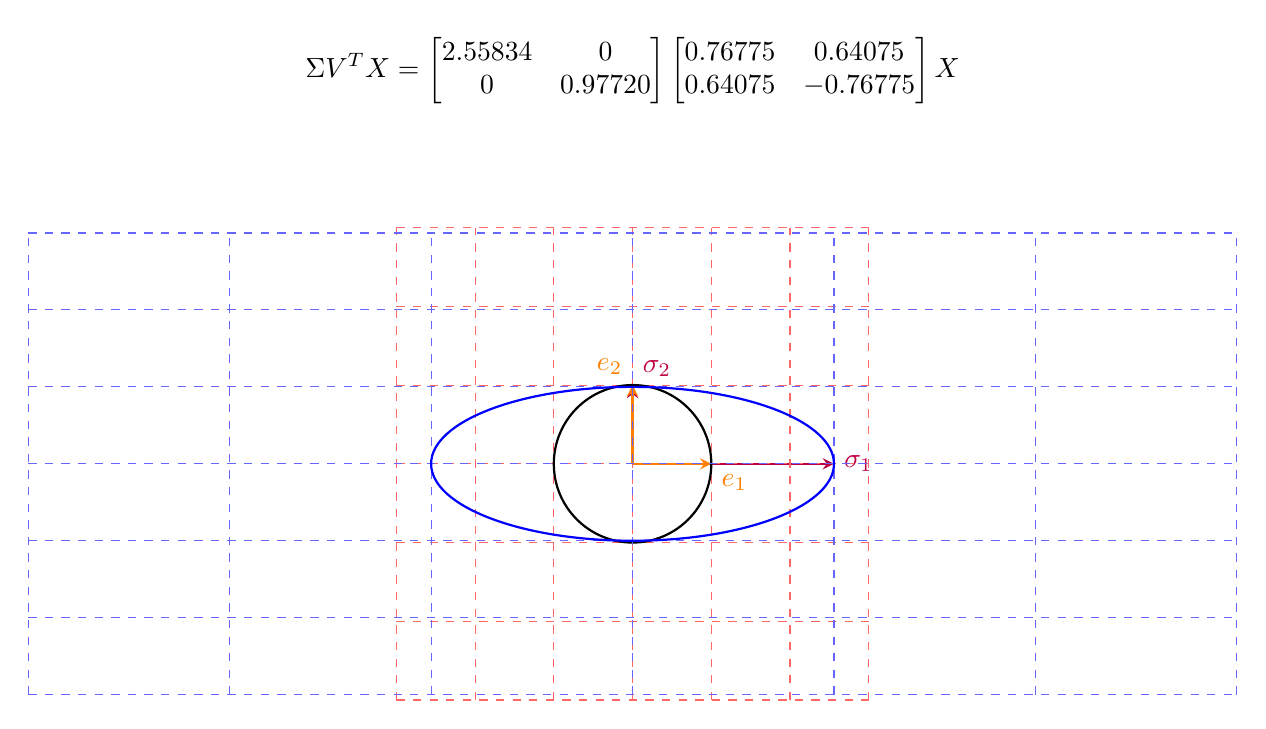
\begin{tikzpicture}% {{{ \Sigma V^T X
	\pgftransformcm{0.76775}{0.64075}{0.64075}{-0.76775}{\pgfpoint{0}{0}}
	\pgftransformcm{0.76775}{0.64075}{0.64075}{-0.76775}{\pgfpoint{0}{0}}
	\draw [thin,red!60, dashed] (-3,-3) grid (3,3);
	\draw[thick, ->, >=stealth, orange] (0,0) -- +(1,0) node[below right]{$e_1$};
	\draw[thick, ->, >=stealth, orange] (0,0) -- +(0,1) node[above left]{$e_2$};
	\draw[thick] (0,0) circle (1);

	\node at (0, 5){$\Sigma V\tp X =\begin{bmatrix}  2.55834 & 0 \\ 0 & 0.97720  \end{bmatrix} \begin{bmatrix}  0.76775 & 0.64075 \\ 0.64075 & -0.76775  \end{bmatrix} X $};

	\pgftransformcm{2.55834}{0}{0}{0.97720}{\pgfpoint{0}{0}}
	\draw [blue!60, thin, dashed] (-3,-3) grid (3,3);
	\begin{scope}[on background layer]
		\draw[thick, ->, >=stealth, purple] (0,0) -- +(1,0) node[right]{$\sigma_1 $};
		\draw[thick, ->, >=stealth, purple] (0,0) -- +(0,1) node[above right]{$\sigma_2 $};
	\end{scope}
	\draw[thick, blue] (0,0) circle (1);
\end{tikzpicture}% }}}

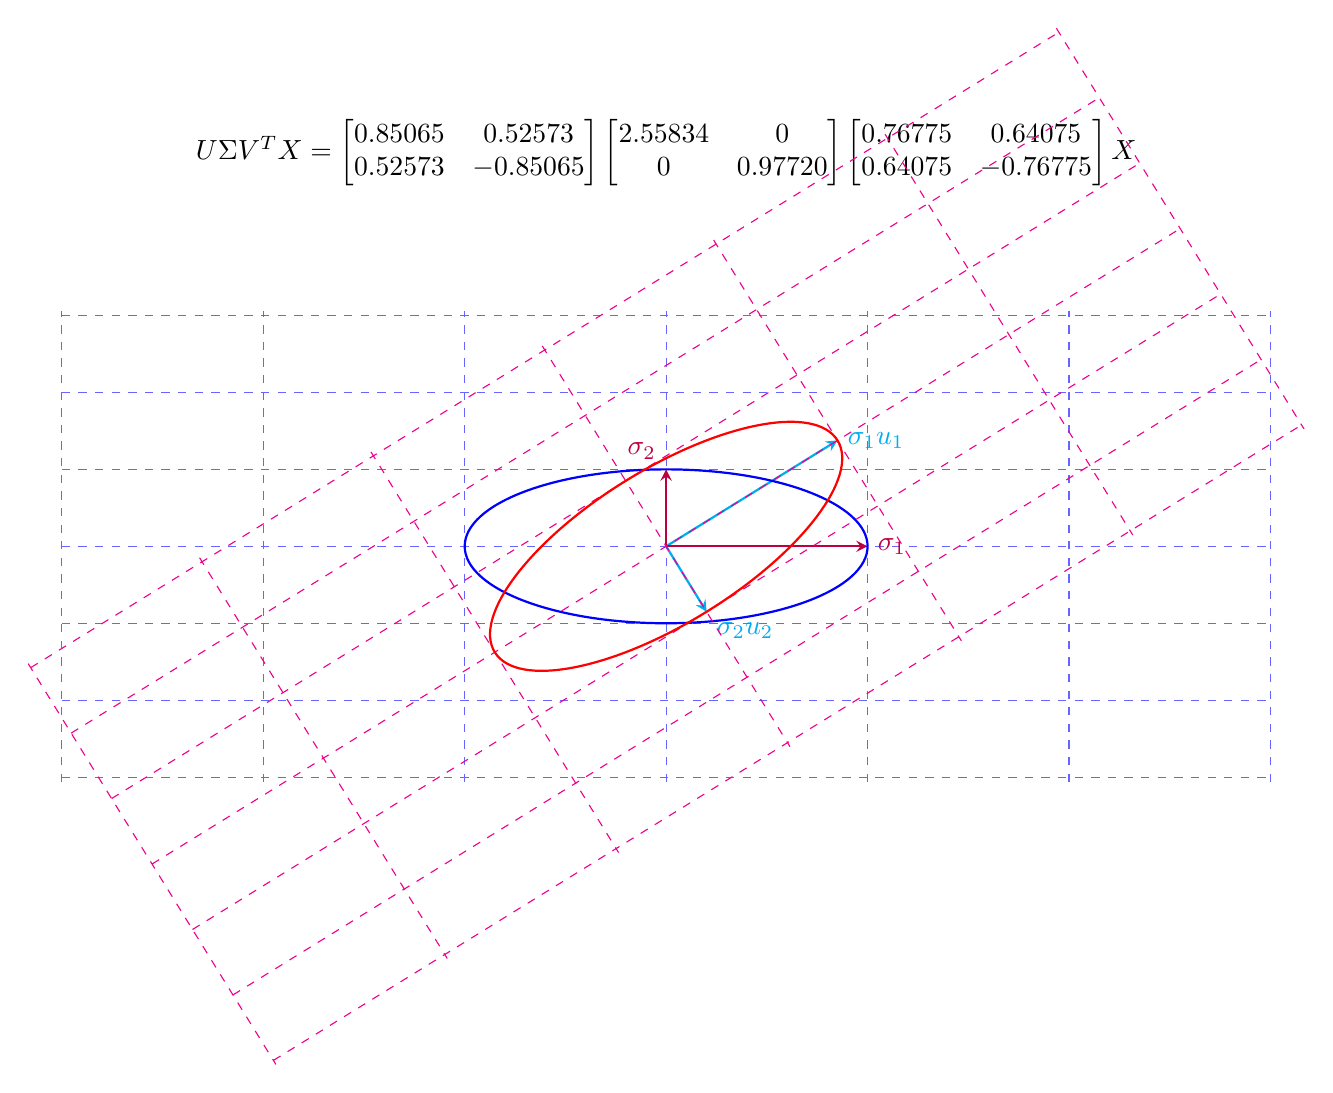
\begin{tikzpicture}% {{{ U \Sigma V^T X
	\draw [thin,blue!60, dashed, xstep=2.55834, ystep=0.97720] (-3*2.55834,-3*0.99720) grid (3*2.55834,3*0.99720);
	\draw[thick, ->, >=stealth, purple] (0,0) -- +(2.55834,0) node[right]{$\sigma_1$};
	\draw[thick, ->, >=stealth, purple] (0,0) -- +(0,0.97720) node[above left]{$\sigma_2$};
	% \draw[thick] (0,0) circle (1);
	\draw[thick, blue] (0,0) ellipse (2.55834 and 0.97720);

	\node at (0, 5){$U\Sigma V\tp X =\begin{bmatrix}  0.85065 & 0.52573 \\ 0.52573 & -0.85065  \end{bmatrix}\begin{bmatrix}  2.55834 & 0 \\ 0 & 0.97720  \end{bmatrix} \begin{bmatrix}  0.76775 & 0.64075 \\ 0.64075 & -0.76775  \end{bmatrix} X $};

	\pgftransformcm{0.85065}{0.52573}{0.52573}{-0.85065}{\pgfpoint{0}{0}}
	\draw [thin,magenta, dashed, xstep=2.55834, ystep=0.97720]  (-3*2.55834,-3*0.99720) grid (3*2.55834,3*0.99720);
	\begin{scope}[on background layer]
		\draw[thick, ->, >=stealth, cyan] (0,0) -- +(2.55834,0) node[right]{$\sigma_1 u_1$};
		\draw[thick, ->, >=stealth, cyan] (0,0) -- +(0,0.97720) node[below right]{$\sigma_2 u_2$};
	\end{scope}
	% \draw[thick, red] (0,0) circle (1);
	\draw[thick, red] (0,0) ellipse (2.55834 and 0.97720);
\end{tikzpicture}% }}}

\begin{tikzpicture}% {{{ AX
	\draw [thin,red!60, dashed] (-3,-3) grid (3,3);
	\draw[thick, ->, >=stealth, orange] (0,0) -- +(1,0) node[right]{$e_1$};
	\draw[thick, ->, >=stealth, orange] (0,0) -- +(0,1) node[above]{$e_2$};
	\draw[thick] (0,0) circle (1);

	\node at (0, 5){$AX =\begin{bmatrix}  2 & 1 \\ 0.5 & 1.5  \end{bmatrix} X $};

	\pgftransformcm{2}{0.5}{1}{1.5}{\pgfpoint{0}{0}}
	\draw [olive, thin, dashed] (-3,-3) grid (3,3);
	\begin{scope}[on background layer]
		\draw[thick, ->, >=stealth, green] (0,0) -- +(1,0) node[right]{$q_1$};
		\draw[thick, ->, >=stealth, green] (0,0) -- +(0,1) node[left]{$q_2$};
	\end{scope}
	\draw[thick, red] (0,0) circle (1);
\end{tikzpicture}% }}}

\end{document}